\section{Datasets}

\subsection{Overview sur les Datasets} 

Les datasets utilisés dans ce projet sont issus du dépôt GitHub de Jinyu Sun et al. \cite{Sun} sur le DeepDonor.
Dans ce dépôt on trouve deux types de datasets : SM (Small Molecules) et PM (Polymer Molecules). Pour pouvoir évalué le modèle plus tard il nous fallait les mêmes données que celles utilisées par Jinyu Sun et al. \cite{Sun}.

Le datset SM est constitué de \textbf{979 SM} tandis que le datasets PM est constitué de \textbf{1285 PM} et comportent des molécules qui proviennent de la littérature.
Ils sont sont au format \textbf{csv} et dans chacun d'eux on retrouve les molécules encodés en \textbf{SMILES} et leurs \textbf{PCE} respectifs.

\begin{figure}[htbp]
    \centering
    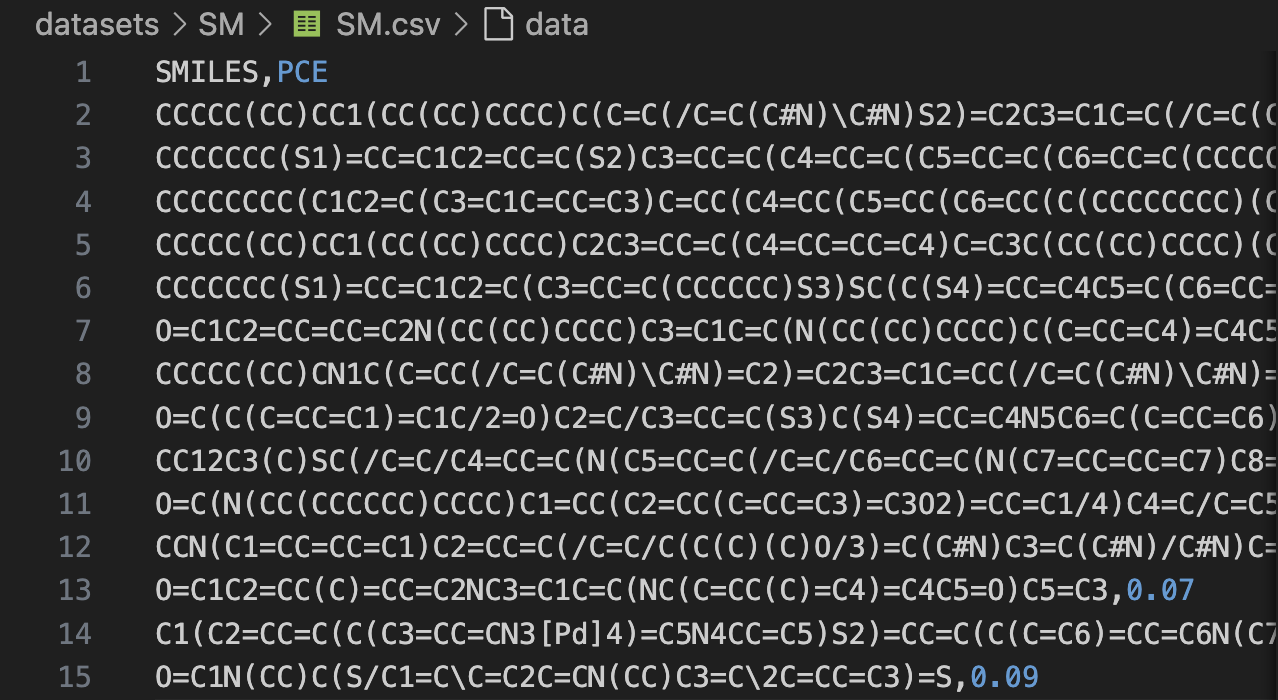
\includegraphics[width=0.6\textwidth]{Datasets/data.png}
    \caption{SMILES et PCE}
\end{figure}

Comme on peut le voir sur la figure ci-dessus, chaque ligne du fichier csv correspond à une molécule encodé en SMILES associées à leurs PCE respectif.

Un point important à noter est le fait qu'il y a une différence entre les PM et les SM. Cette différence réside au niveau de la masse moléculaires.
Ainsi, ce point est intéressant à prendre en compte pour éviter toute confusion pour la suite.

\subsection{Datasets de coordonnées 3D}

Les datasets évoqués précédement servent de point d'entrée pour le modèle de prédiction (Quantum Deep Field).
Pour permettre au modèle de prédiction de capter la structure moléculaires des molécules il faut des données numériques d'où l'idée de transformer les SMILES en coordonnées 3D. 
De plus, à partir de ces données numériques ils pourraient être possibles de prédire d'autres propriétés électroniques liés aux molécules. 

\begin{figure}[H]
    \centering
    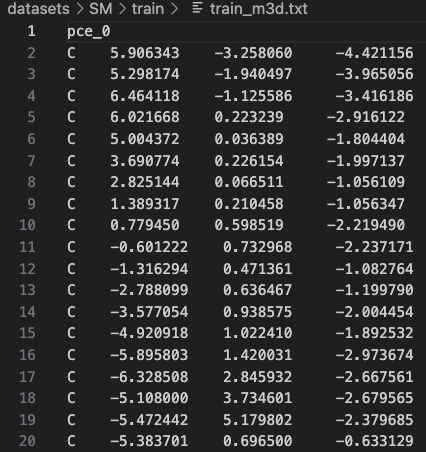
\includegraphics[width=0.4\textwidth]{Datasets/coords.png}
    \caption{Coordonnées 3D d'une molécule}
\end{figure}

Pour chaque molécules, on génére les coordonnées 3D de chaque atomes.
Ensuite on récupère ces coordonnées 3D on effectue un prétraitement  pour les transformer en fichier \texttt{.npy} pour qu'ils puissent enfin être utilisé par le modèle de prédiction.


